\Chapter{Background e Stato dell'Arte}


La segmentazione semantica di immagini mediche rappresenta una delle sfide più importanti nel campo della diagnostica. Questo compito, che consiste nel delineare con precisione \textbf{strutture anatomiche} o \textbf{aree patologiche} all’interno di \textbf{immagini biomediche}, ha un impatto diretto su applicazioni cliniche cruciali come la pianificazione chirurgica e il monitoraggio terapeutico. Nel contesto specifico della \textbf{mammella}, la segmentazione da immagini \textbf{MRI 3D} presenta peculiarità che la rendono particolarmente \textbf{complessa}, tra cui l’elevata \textbf{variabilità anatomica tra pazienti}, la presenza di \textbf{artefatti tipici delle risonanze magnetiche} e la necessità di bilanciare \textbf{accuratezza} e \textbf{tempi di elaborazione} quando si lavora con volumi tridimensionali ad alta risoluzione.

\Section{L’Evoluzione delle Tecniche di Segmentazione}

Prima dell’avvento del \textbf{deep learning}, la segmentazione di immagini mediche si basava principalmente su approcci tradizionali che, pur rappresentando soluzioni pionieristiche per l’epoca, presentavano limiti significativi. Tecniche come il \textbf{thresholding} e il \textbf{region-growing}, ad esempio, erano ampiamente utilizzate per la loro semplicità concettuale, ma risultavano estremamente sensibili alla qualità dell’immagine, fallendo spesso in presenza di rumore o basso contrasto tra i tessuti. Allo stesso modo, i \textbf{deformable models}, che cercavano di adattare contorni attivi alle strutture anatomiche, richiedevano un’inizializzazione manuale e faticavano a gestire la complessa morfologia della ghiandola mammaria.

Con l’introduzione delle reti \textbf{neurali convoluzionali} (\textbf{CNN}), il panorama della segmentazione medica è cambiato radicalmente. L’architettura \textbf{U-Net}, proposta nel 2015 da \textbf{Ronneberger et al.,} ha rappresentato una svolta grazie alla sua struttura \textbf{encoder-decoder} e alle \textbf{skip connections}, che permettono di combinare informazioni a diversi livelli di risoluzione, preservando i dettagli spaziali fondamentali per una segmentazione precisa. Successivamente, la comunità scientifica ha sviluppato varianti sempre più avanzate, come la \textbf{V-Net}, ottimizzata per dati volumetrici, e il framework \textbf{nnU-Net}, in grado di adattarsi automaticamente alle caratteristiche di diversi dataset medici.

Negli ultimi anni, l’attenzione si è spostata verso i \textbf{Transformers}, modelli nati nell’ambito del \textbf{Natural Language Processing} e poi adattati con successo all’analisi di immagini. Architetture come \textbf{TransUNet} e \textbf{Swin UNETR} combinano la capacità delle CNN di estrarre features locali con il potere dei Transformers di modellare relazioni globali, offrendo prestazioni superiori in molti task di segmentazione. Tuttavia, questi modelli richiedono risorse computazionali elevate e grandi quantità di dati annotati, il che ne limita ancora l’applicabilità in alcuni contesti clinici.


\Section{Architettura U-Net per la Segmentazione di Immagini Mediche}

Tra le architetture più utilizzate nel campo della segmentazione semantica applicata all’imaging biomedico, la \textbf{U-Net} occupa senza dubbio un ruolo di primo piano. Introdotta da \textbf{Ronneberger et al. nel 2015}, questa rete è stata progettata appositamente per segmentare immagini mediche anche in condizioni di \textbf{disponibilità limitata di dati annotati,} un aspetto ricorrente nei contesti clinici reali. Il successo della U-Net è dovuto non solo alla sua efficacia, ma anche alla sua semplicità architetturale, che la rende estremamente versatile e facilmente adattabile a diverse tipologie di dati, tra cui immagini 2D, 3D o multi-canale.

L'architettura della U-Net si sviluppa secondo una struttura simmetrica a forma di U \ref{fig:Schema concettuale dell'architettura U-Net}, composta da due fasi principali: un percorso di \textbf{contrazione}, o encoder, e un percorso di \textbf{espansione}, o decoder. La fase di contrazione ha il compito di \textbf{estrarre rappresentazioni sempre più astratte} e semantiche dell’immagine in input, riducendone progressivamente la risoluzione attraverso \textbf{convoluzioni} e operazioni di \textbf{pooling}. Al contrario, la fase di espansione mira a \textbf{ricostruire l’informazione spaziale originaria}, riportando l’output alla dimensione dell’immagine di partenza mediante operazioni di \textbf{upsampling} e \textbf{convoluzioni}.

\begin{figure}[H]
  	\centering 
 	\includegraphics[width=.6\textwidth]{figures/U-Net-architecture.png} 
	 \caption{Schema concettuale dell'architettura U-Net.}
	 \label{fig:Schema concettuale dell'architettura U-Net}
	\end{figure} 

Una caratteristica distintiva della U-Net rispetto ad altre reti di segmentazione è la presenza delle cosiddette \textbf{skip connections}. Questi collegamenti diretti tra i livelli corrispondenti \textbf{dell’encoder} e del \textbf{decoder} permettono di trasportare le informazioni a bassa astrazione, spesso perse durante il downsampling, direttamente nei livelli di ricostruzione. In questo modo, la rete riesce a \textbf{combinare efficacemente il contesto globale} dell’immagine con i \textbf{dettagli locali}, migliorando significativamente la \textbf{precisione dei bordi} e la \textbf{definizione delle strutture segmentate}.

Dal punto di vista pratico, la U-Net prende in input un’immagine e produce come output una \textbf{maschera segmentata}, in cui ogni pixel (o voxel nel caso 3D) è classificato in una determinata categoria. Questo rende la rete particolarmente adatta per compiti dove è richiesta una \textbf{segmentazione voxel-wise}, come nel caso dell’identificazione di tessuti, lesioni o strutture anatomiche specifiche.

% Nel progetto descritto in questa tesi, la U-Net è stata adottata come architettura di base per la segmentazione automatica del seno e del tessuto fibroghiandolare in immagini MRI. Questo approccio è ispirato anche al lavoro recente di \textbf{Lew et al. (2024),} in cui \textbf{due reti U-Net} sono state combinate in cascata per segmentare prima il seno intero e successivamente il tessuto interno, comprendente FGT e vasi sanguigni. 

In tal senso, la U-Net si è dimostrata una \textbf{scelta solida}, grazie alla sua capacità di generalizzare anche su strutture anatomiche complesse, pur mantenendo una buona efficienza computazionale, ma nonostante la sua efficacia, la U-Net presenta alcune \textbf{limitazioni}. In presenza di \textbf{rumore}, \textbf{artefatti} o \textbf{grandi squilibri tra le classi}, la rete può mostrare difficoltà, ad esempio nel riconoscere strutture piccole o nel distinguere tessuti contigui con caratteristiche simili. Per superare tali difficoltà, sono state sviluppate diverse \textbf{estensioni} e \textbf{varianti} dell’architettura originale, come \textbf{l’U-Net++} con connessioni più profonde, le \textbf{U-Net con meccanismi di attention}, o le versioni 3D per dati volumetrici. Tuttavia, anche nella sua forma standard, la U-Net continua a rappresentare un punto di partenza solido e affidabile per molte applicazioni di segmentazione in ambito medico.




\Section{Strumenti e Dataset Moderni}
Oggi, lo sviluppo di pipeline per la segmentazione medica si avvale di strumenti sempre più sofisticati. Tra questi, il framework \textbf{MONAI} (\textbf{Medical Open Network for AI}) si è affermato come uno standard de facto, grazie alla sua vasta raccolta di trasformazioni specifiche per immagini mediche, modelli predefiniti e metriche di valutazione. Basato su \textbf{PyTorch}, MONAI semplifica notevolmente la gestione di dati complessi come quelli DICOM e supporta l’implementazione di workflow riproducibili, essenziali per la ricerca in ambito medico.

Per quanto riguarda i dataset, il \textbf{Duke-Breast-Cancer-MRI} \cite{duke_breast_mri}, disponibile su \textbf{The Cancer Imaging Archive (TCIA),} rappresenta una risorsa preziosa per lo studio della segmentazione mammaria. Questo dataset include volumi MRI multiparametrici annotati manualmente da radiologi esperti, catturando tutta la complessità anatomica e le sfide tipiche delle immagini reali, come la presenza di lesioni e la variabilità nella densità del tessuto.


\Section{Stato dell'Arte nella Segmentazione del Seno in MRI 3D}
Come già accennato, negli ultimi anni, la segmentazione automatica delle immagini mediche ha ricevuto un crescente interesse grazie all’utilizzo di reti neurali convoluzionali (CNN), in particolare per compiti complessi come l’analisi della densità mammaria. Uno studio di riferimento in questo ambito è quello di \textbf{Lew et al. (2024)} \cite{lew2024segmentation}, che ha proposto un modello basato su U-Net per la segmentazione automatica del seno, del tessuto fibroghiandolare (FGT) e dei vasi sanguigni su risonanza magnetica (MRI) pre-contrasto \ref{fig:schema_segmentazione_seno_paper}.

\begin{figure}[H] 
  	\centering 
 	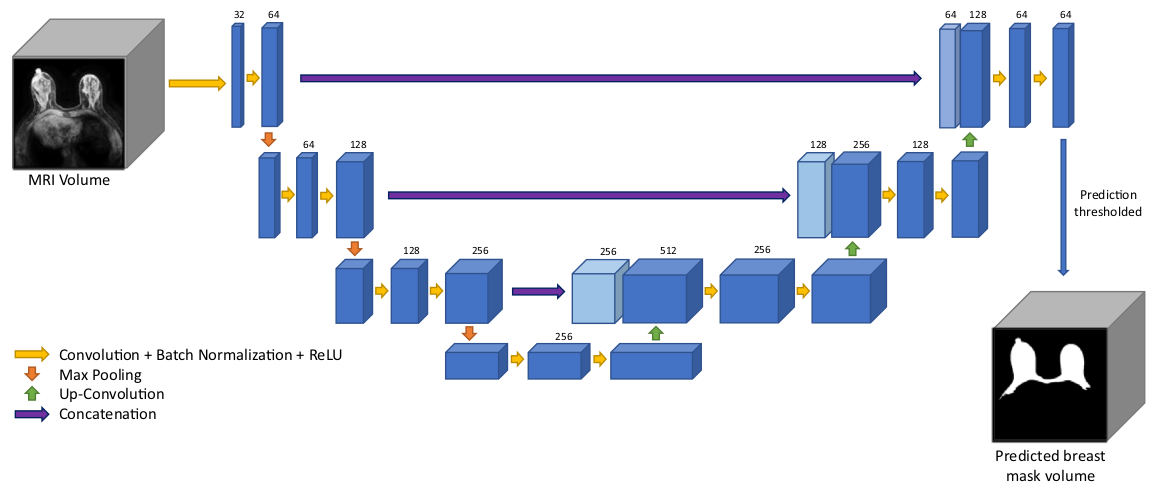
\includegraphics[width=\textwidth]{images/2025-07-07-12-01-04.png} 
	 \caption{Overview dei dati di input e la U-NET usata per la segmentazione del seno.}
    \label{fig:schema_segmentazione_seno_paper}
 \end{figure} 

Il lavoro si distingue per l’approccio rigoroso e riproducibile all’annotazione dei dati: \textbf{100 studi MRI}, selezionati dal già citato dataset pubblico \textit{Duke Breast Cancer MRI} \cite{duke_breast_mri}, sono stati annotati manualmente seguendo criteri ben definiti e validati da radiologi specializzati. Le annotazioni sono tridimensionali e comprendono il \textbf{tessuto mammario}, il \textbf{FGT} e i \textbf{vasi}, un elemento spesso trascurato in studi precedenti.

Dal punto di vista architetturale, il sistema utilizza \textbf{due reti U-Net in cascata}:
\begin{itemize}
\item \textbf{Breast U-Net}, che segmenta il tessuto mammario nell’intero volume MRI.
\item \textbf{FGT-Vessel U-Net}, che utilizza sia il volume MRI che la segmentazione del seno come input per individuare il FGT e i vasi sanguigni.
\end{itemize}

Le performance sono state valutate tramite il \textbf{coefficiente di similarità di Dice (DSC)}, ottenendo i seguenti risultati medi sul test set:
\begin{itemize}
\item \textbf{Breast segmentation:} DSC = \hlight{0.92 (3D), 0.95 (2D)}
\item \textbf{FGT segmentation: DSC} = \hlight{0.86 (3D), 0.84 (2D)}
\item \textbf{Blood vessels: DSC} = \hlight{0.65 (3D), 0.53 (2D)}
\end{itemize}

Un elemento innovativo del lavoro è la \textbf{segmentazione esplicita dei vasi}, che ha mostrato impatto significativo nella stima della densità mammaria. In effetti, \textbf{il volume dei vasi rappresentava in media il 5.7\% del totale dei voxel etichettati come FGT o vasi.} Trascurare questo aspetto, come avveniva in studi precedenti, può portare a una sovrastima della densità mammaria.

% \Section{Le Sfide Aperte}
% Nonostante i progressi compiuti, la segmentazione del seno in MRI 3D presenta ancora diverse criticità. Una delle principali è la scarsità di dataset pubblici di grandi dimensioni, soprattutto se confrontata con la disponibilità di dati per altri organi come il cervello o il fegato. Inoltre, i modelli esistenti faticano spesso a generalizzare su dati provenienti da diversi centri medici, a causa delle variazioni tra scanner e protocolli di acquisizione.

% Un altro aspetto critico è l’integrazione di questi strumenti nei workflow clinici quotidiani. Molti modelli, pur offrendo prestazioni elevate in contesti sperimentali, non sono ancora ottimizzati per l’uso in tempo reale o per interagire con i sistemi informativi ospedalieri. Infine, la mancanza di interpretabilità delle predizioni rimane un ostacolo significativo per l’adozione clinica, poiché i medici necessitano di comprendere le basi delle decisioni algoritmiche.

% Questo contesto evidenzia l’importanza di sviluppare soluzioni innovative che affrontino non solo gli aspetti tecnici della segmentazione, ma anche le esigenze pratiche degli operatori sanitari. La pipeline proposta in questo lavoro si inserisce proprio in questo spazio, cercando di colmare alcune delle lacune esistenti attraverso un approccio bilanciato tra accuratezza, efficienza e adattabilità.